\documentclass[a4paper,12pt]{article}
\usepackage[ngerman]{babel}
\usepackage{ucs}
\usepackage{multirow}
\usepackage{xltxtra}
\usepackage[utf8x]{inputenc}
\usepackage{fontspec}
\usepackage{eurosym}
\usepackage{graphicx}
\usepackage[paper=a4paper,left=25mm,right=25mm,top=25mm,bottom=25mm]{geometry}
\usepackage{makecell}
\usepackage[table]{xcolor}
\usepackage{float}
\usepackage[normalem]{ulem}
\usepackage{xcolor,colortbl}
\definecolor{Gray}{gray}{0.85}
\usepackage[automark]{scrlayer-scrpage}
\pagestyle{scrheadings}
\clearscrheadfoot
\setmainfont[Mapping=tex-text]{Liberation Serif}
\begin{document}
\input{version.tex}
\ohead{Regelstand: \commitDate, id: \commitID}
\title{\tagYear\ Line Following Challenge Regeln}
\makeatletter
\let\inserttitle\@title
\makeatother
\begin{center}
	
\includegraphics[width=0.5\textwidth]{logo.png}

	\huge                      % Schriftgröße einstellen
	\bfseries                   % Fettdruck einschalten
	\inserttitle
\end{center}

\section{Ziel}
Entwerfe, konstruiere und programmiere einen Linienfolge-Roboter, der (in drei
Minuten) einer schwarzen Linie auf weißem Hintergrund zu einem Turm folgen und
mindestens einen (1) Ball abgeben und dann zu seinem Ausgangspunkt zurückkehren
kann. In der verbleibenden Zeit kehrt er zum Turm zurück (so oft wie nötig), um
eine bestimmte Anzahl (nicht über oder unter) von Bällen gemäß den Vorgaben der
jeweiligen Altersgruppe des Teams abzugeben.

\section{Altersgruppen}

Die Teams dieser Challenge treten in unterschiedlichen Altersgruppen an:
\begin{itemize}
	\item ES
	\item MS
	\item HS
	\item UP
\end{itemize}

\section{Anforderungen}
Autonomer Roboter, basierend auf beliebiger Plattform, der \euro{1.500}  oder
weniger kostet und die folgenden Designbedingungen erfüllt, die beim Check-In
überprüft werden:
\begin{itemize}
	\item Der Roboter kann auf einer Teststrecke demonstrieren, dass er
		ein Linienfolge-Programm ausführt.
	\item Der Roboter kann demonstrieren, dass er beim Erreichen des Turms
		anhält; es muss nicht nachgewiesen werden, dass er eine Kugel
		auswerfen oder sich umdrehen kann.
	\item Mehrere Sensoren und Prozessoren sind erlaubt.
	\item Das Volumen des Roboters darf 65030 cm3 nicht überschreiten.
\end{itemize}

\section{Allgemeine Spielregeln}
\begin{itemize}
	\item Der Veranstalter legt die Anzahl der erlaubten offiziellen Läufe
		fest und die Anzahl dieser offiziellen Läufe, die für die
		Gesamtpunktzahl gezählt werden, die zur Ermittlung der
		Top-8-Teams, die an dem Turnier teilnehmen werden, verwendet
		wird.
	\item Der Roboter hat 3 Minuten Zeit, um diese Aufgaben zu erledigen.
	\item Ein Linienfolgeprogramm muss die Bewegung Deines Roboters zu
		jeder Zeit kontrollieren.
		%can?
	\item Nur die Spieler dürfen den Roboter während des Laufs bedienen und
		handhaben. Denkt daran: ``Spieler spielen, Trainer trainieren,
		Eltern jubeln''.
	\item Der Turm darf während der Auslieferung der Nutzlast von niemandem
		berührt werden.
	\item \textbf{Kein Herausschaufeln von Kugeln aus dem Turm durch eine
		Person während der Auslieferung der Nutzlast.}
	\item Wenn der Roboter zu irgendeinem Zeitpunkt berührt wird, muss er
		hochgehoben und zum Startpunkt zurückgebracht werden.
\end{itemize}

\section{Spezifikationen des Challenge Equipments}

\subsection{Der Turm}
Größenangaben sind Richtwerte von denen es leichte Abweichungen geben kann.
\begin{itemize}
	\item Alle Altersgruppen benutzen 20 cm hohen x 10 cm breiten x 35 cm
		langen Turm mit einer 10×10 cm großen Öffnung an der Oberseite
		und einer offenen Rückwand, aus der die Bälle bei der
		Auslieferungen herausrollen können. Der Karton ist mit
		Klebeband am Spielplan fixiert.
	\item Wenn ein Punktrichter sieht, dass ein Team Mitglied den Turm
		berührt oder in diesen hineingreift, wird der Lauf abgebrochen
		und das Team bekommt nur 400 Punkte für das Absolvieren des
		Challenge Parcours unabhängig davon wieviele Bälle ausgeliefert
		wurden.
\end{itemize}
\subsection{Der Spielplan}
\begin{itemize}
	\item Die Spielpläne werden üblicherweise auf stabilem Papier oder PVC-Plane gedruckt.
	\item Altersgruppe ES – Keine Abzweigungen, 1,25 cm schwarze Linie
	\item Altersgruppe MS – Eine Abzweigung, 1,25 cm schwarze Linie
	\item Altersgruppen HS \& BK – Zwei Abzweigungen, 0,75 cm schwarze Linie
	\item Jedes Jahr wird ein neues Design erstellt
	\item Es führen mindestens 20 cm gerade Linie direkt zum Turm hin
	\item Die Linie wird nicht weniger als 10 cm vom Rand des Spielplanes
		oder von irgendeiner anderen Linie entfernt sein
	\item Werbung oder gedruckte Anweisungen können überall auf dem
		Spielplan platziert sein, müssen aber einen Abstand von
		mindestens 10 cm zu den Linien einhalten.
	\item Die Kurven können sich im Radius unterscheiden, aber keine Kurve
		darf einen Radius kleiner als 15 cm für die Altersgruppe MS oder 10 cm für die
		Altersgruppen HS und UP haben.
\end{itemize}
\subsection{Spielplan Beispiele}
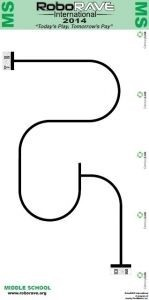
\includegraphics[width=0.3\textwidth]{track_ms_lf.png}
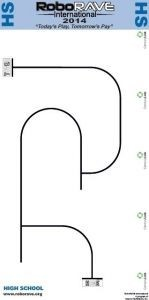
\includegraphics[width=0.3\textwidth]{track_hs_lf.png}
\emph{Die abgebildeten Spielpläne sind \textbf{Beispiele}. Das Design ändert sich von Jahr zu
Jahr und wird am ersten Tag des Wettbewerbes veröffentlicht.}
\subsection{Andere wichtige Punkte }
\begin{itemize}
	\item Die Challenge kann an Orten mit natürlichen Licht stattfinden
		welches die Lichtverhältnisse auf dem Spielplan verändert.
		Teams sollten darauf vorbereitet sein, diese natürlichen
		Bedingungen zu meistern.
	\item Die Veranstaltungsleitung kann entscheiden den HS Spielplan für
		die Altersgruppe UP zu verwenden oder einen schwierigeren
		Spielplan zu erstellen. Außerdem kann die Öffnung des Turms für
		die Altersgruppe UP verkleinert werden
\end{itemize}
\section{Punktevergabe}
Die Gesamtpunktzahl ist die Summe der Punkte aus:
\begin{itemize}
	\item Absolvieren des Parcours zum Turm
	\item Ausliefern von mindestens einem Ball
	\item Rückkehr des Roboters zum Ausgangspunkt
	\item Wiederholtes Absolvieren des Parcours so oft bis die
		erforderliche Anzahl an Bällen augeliefert wurde
\end{itemize}

Jede Altersgruppe hat eine vorgegebene Anzahl an Bällen auszuliefern. Die
Zahlen werden am Tag des Wettbewerbes veröffentlicht. Dies sind die Bereiche
aus welchen die Anzahl Bälle der Altersgruppen gewählt sein müssen:
\begin{itemize}
	\item Altersgruppe ES - zwischen 75 und 125 Bällen
	\item Altersgruppe MS - zwischen 125 und 200 Bällen
	\item Altersgruppe HS – zwischen 200 und 250 Bällen
	\item Altersgruppe UP - zwischen 100 und 350 Bällen (die Zahl ist
		niedrig sollte die Öffnung des Turms verkleinern sein)
\end{itemize}

Die Anzahl Punkte die für die erste Fahrt zum Turm und zurück in den
entsprechenden Altersgruppe vergeben werden, kann der untenstehenden
Punktetabelle entnommen werden.

\subsection{Ein erfolgreicher Lauf ist wie folgt definiert:}
\begin{itemize}
	\item Der Roboter absolviert den Parcour vom Startpunkt zum Turm,
		liefert mindestens einen Ball aus und kehrt entlang des
		Parcours wieder zum Ausgangspunkt zurück. Alle während dieses
		Durchlaufs ausgelieferten Bälle werden entfernt und werden
		nicht als Bonuspunkte gezählt
	\item Es kann mehrerer Versuche bedürfen die oben genannten Aufgaben zu
		erledigen. Sobald alle Aufgaben erledigt wurden, können die
		Teams Bonuspunkt Läufe durchführen.
	\item Bei einem Bounspunkt Lauf absolviert der Roboter den Parcours vom
		Startpunkt zum Turm und liefert die in der Altersgruppe
		geforderte Anzahl Punkte aus. Während der Bonuspunkt Läufe muss
		der Roboter nicht dem Parcours vom Turm zurück zum Startpunkt
		folgen
\end{itemize}
\subsection{Punktevergabe beim Ausliefern von Bonusbällen}
\begin{itemize}
	\item Wenn die Anzahl der Bälle unter der erforderlichen Anzahl Bälle
		liegt, ist die die Anzahl der Bonuspunkte
	\item Wenn die Anzahl der Bälle über der erforderlichen Anzahl Bälle
		liegt, dann wird der Überschuss von der erforderlichen Anzahl
		abgezogen und das Ergebnis ist die die Anzahl der Bonuspunkte
\end{itemize}
\section{Punktetabelle}
\begin{center}
	\begin{tabular}{|c|c|c|c|c|c|} \hline
		\multirow{3}*{} & Verlässt & Passiert erste & Passiert zweite & Stoppt vor dem & Liefert einen \\
		& Startpunkt & Abzweigung & Abzweigung & Karton & Ball zum Karton \\ \hline
		ES & 50 & k.A & k.A & 100 & 100 \\ \hline
		MS & 25 & 25 & k.A & 100 & 100 \\ \hline
		HS/UP & 25 & 25 & 25 & 50 & 100 \\ \hline
	\end{tabular}
	\begin{tabular}{|c|c|c|c|c|c|} \hline
		\multirow{3}*{} & Startet den & Passiert erste & Passiert zweite & Kommt am & Gesamt \\
		& Rückweg & Abzweigung & Abzweigung & Startpunkt an &  \\ \hline
		MS & 50 & k.A. & k.A. & 100 & 400 \\ \hline
		MS & 25 & 25 & k.A. & 100 & 400 \\ \hline
		HS/UP & 25 & 25 & 25 & 100 & 400 \\ \hline
	\end{tabular}
\end{center}
\section{Tunierplan}
\begin{itemize}
        \item Die besten acht Mannschaften werden an der Endrunde teilnehmen.
        \item Die aufsteigenden Teams werden entsprechend ihrer Gesamtpunktzahl in die Turnierliste gesetzt (siehe untenstehende Tabelle).
        \item Der zweite Platz ("`Runner Up"') wird verwendet, um den 3. Platz auf der Grundlage des Ergebnisses der Halbfinalrunde zu bestimmen.
\end{itemize}
\begin{figure}[H]
    \centering
    \def\svgwidth{\columnwidth}
    \input{tournament_score/tournament_score.pdf_tex}
\end{figure}
\end{document}
